\chapter{Progress and Reflection}

This chapter illustrates various aspects reside in the management of the project, including a revision of the original workplan, a description of the working methodology, resource management details and contingency measures. A personal reflection to the project during its first half is also presented. 

\section{Project Management}
% Covering the tasks as a part of your work plan and progress as well as how time and resources are managed.

\subsection{Revision of Workplan}
% Revision of workplan.
Figure \ref{fig:Gantt_old} shows the proposed workplan of the project designed at the beginning stage. Generally speaking, the progress of the project has been satisfying, as all the phases involving literature review and systematic learning have been completed on time. One task was shelved and left behind schedule, however, namely the delivery of an ontology matching framework, which was supposed to come along with the interim report. There are two primary contributing factors to the making of this decision. Firstly, the workload in studying existing ontology matching techniques was underestimated, making the expectation of designing the framework simultaneously with the learning process unrealistic. Secondly, time allocation was inevitably tilted to the investigation of instance matching strategies, as they are inseparable from the general ontology matching framework. This was considered better for the selection of suitable framework components after some investigation into ontology matching, and was hence given higher priority.
\\\\
In order to reflect the above changes, a revised workplan was designed and presented in figure \ref{fig:Gantt_new}. The project is currently at the milestone of Interim Report, and the progress until present is demonstrated in the previous stages. Due to the effect of exam preparation, implementation tasks before the exams are only preliminary, while the major development tasks are put in the winter vacation. This is sensible because coding and debugging can take a large amount of time. The adjustment of instance matching algorithm is now side by side with testing and evaluation, with the validation of design carried all along the way. In the case of unexpected obstacles or potential risks such as increased academic workload during the spring semester, the adjustment phase can shrink to buffer the impact on the overall workplan. The workload of writing the final dissertation is spread over a longer timespan, as it was discovered that writing usually takes longer than expected.

\begin{figure}[ht]
\begin{subfigure}[ht]{\textwidth}
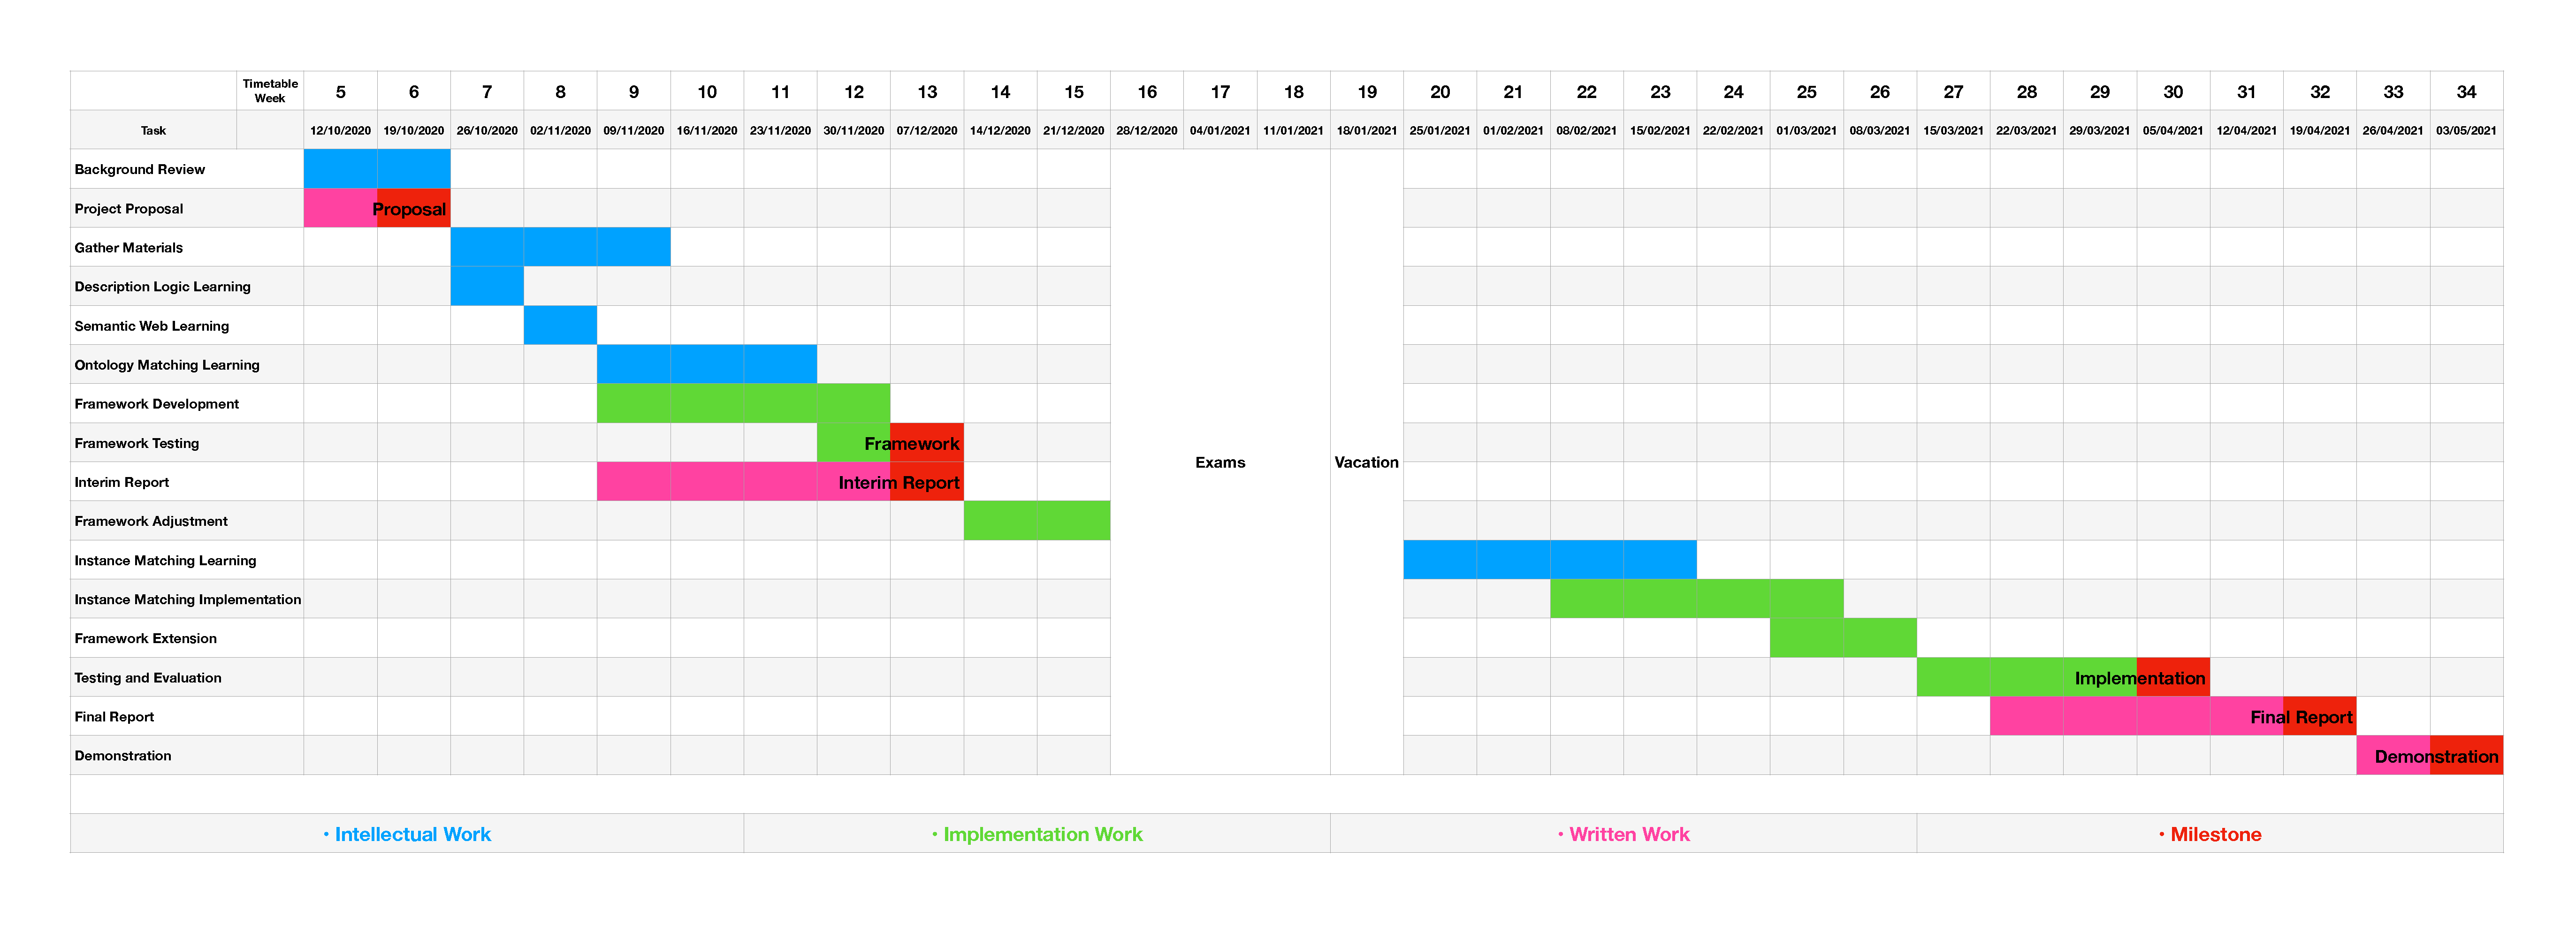
\includegraphics[width=\textwidth]{img/Gantt_old.pdf}
\caption{Original workplan}
\label{fig:Gantt_old}
\end{subfigure}
\begin{subfigure}[ht]{\textwidth}
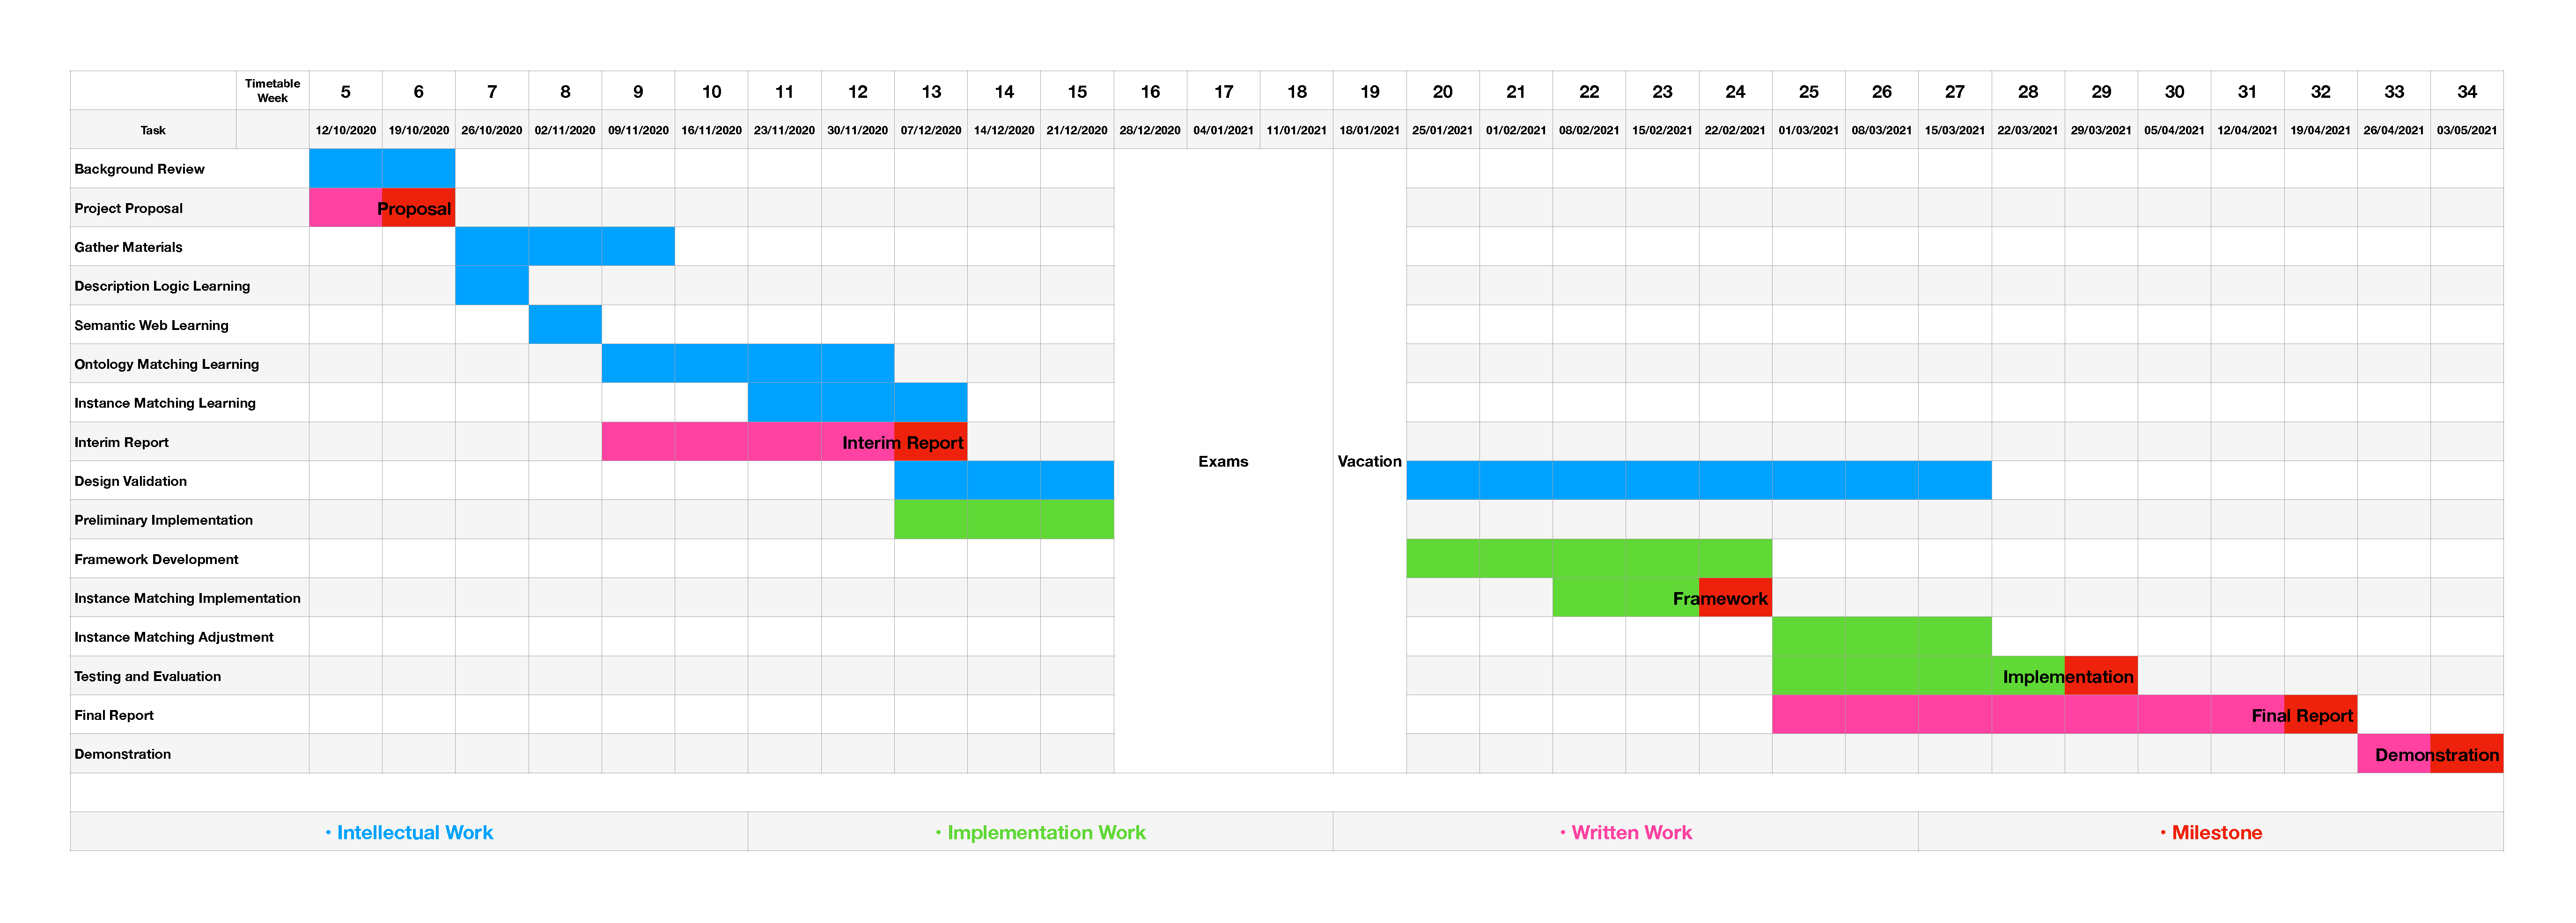
\includegraphics[width=\textwidth]{img/Gantt_new.pdf}
\caption{Revised workplan}
\label{fig:Gantt_new}
\end{subfigure}
\caption{Revision of workplan}
\label{fig:Gantt}
\end{figure}

\subsection{Working Methodology}
% Scrumban methodology.
While the workplan is designed with respect to the Waterfall methodology \cite{balaji2012waterfall} for clear validation of progress against the milestones, a hybrid combination of the Scrum and Kanban methodologies, namely Scrumban \cite{DBLP:conf/ispw/NikitinaKS12}, was adopted and followed as the working methodology since the beginning. The Scrum aspect splits the workload into small, easily achievable goals which could be reviewed regularly, while a Kanban board enables clear monitoring of the process, with tasks being assigned in dynamic "lanes" (see figure \ref{fig:Kanban}). Fusing the two together exploits the advantages of both: the workflow can adapt to changes quickly, and since all tasks are visualised, the efforts can be well balanced and coordinated. The sprint interval for Scrumban was set to 1 week, which is the interval between every consecutive meetings with my supervisor. This helped tremendously in pushing everything forward, so that the project can progress at a good pace despite the intense curricular work during the fall semester and my lack of experience in carrying out a large project like this individually.

\begin{figure}[ht]
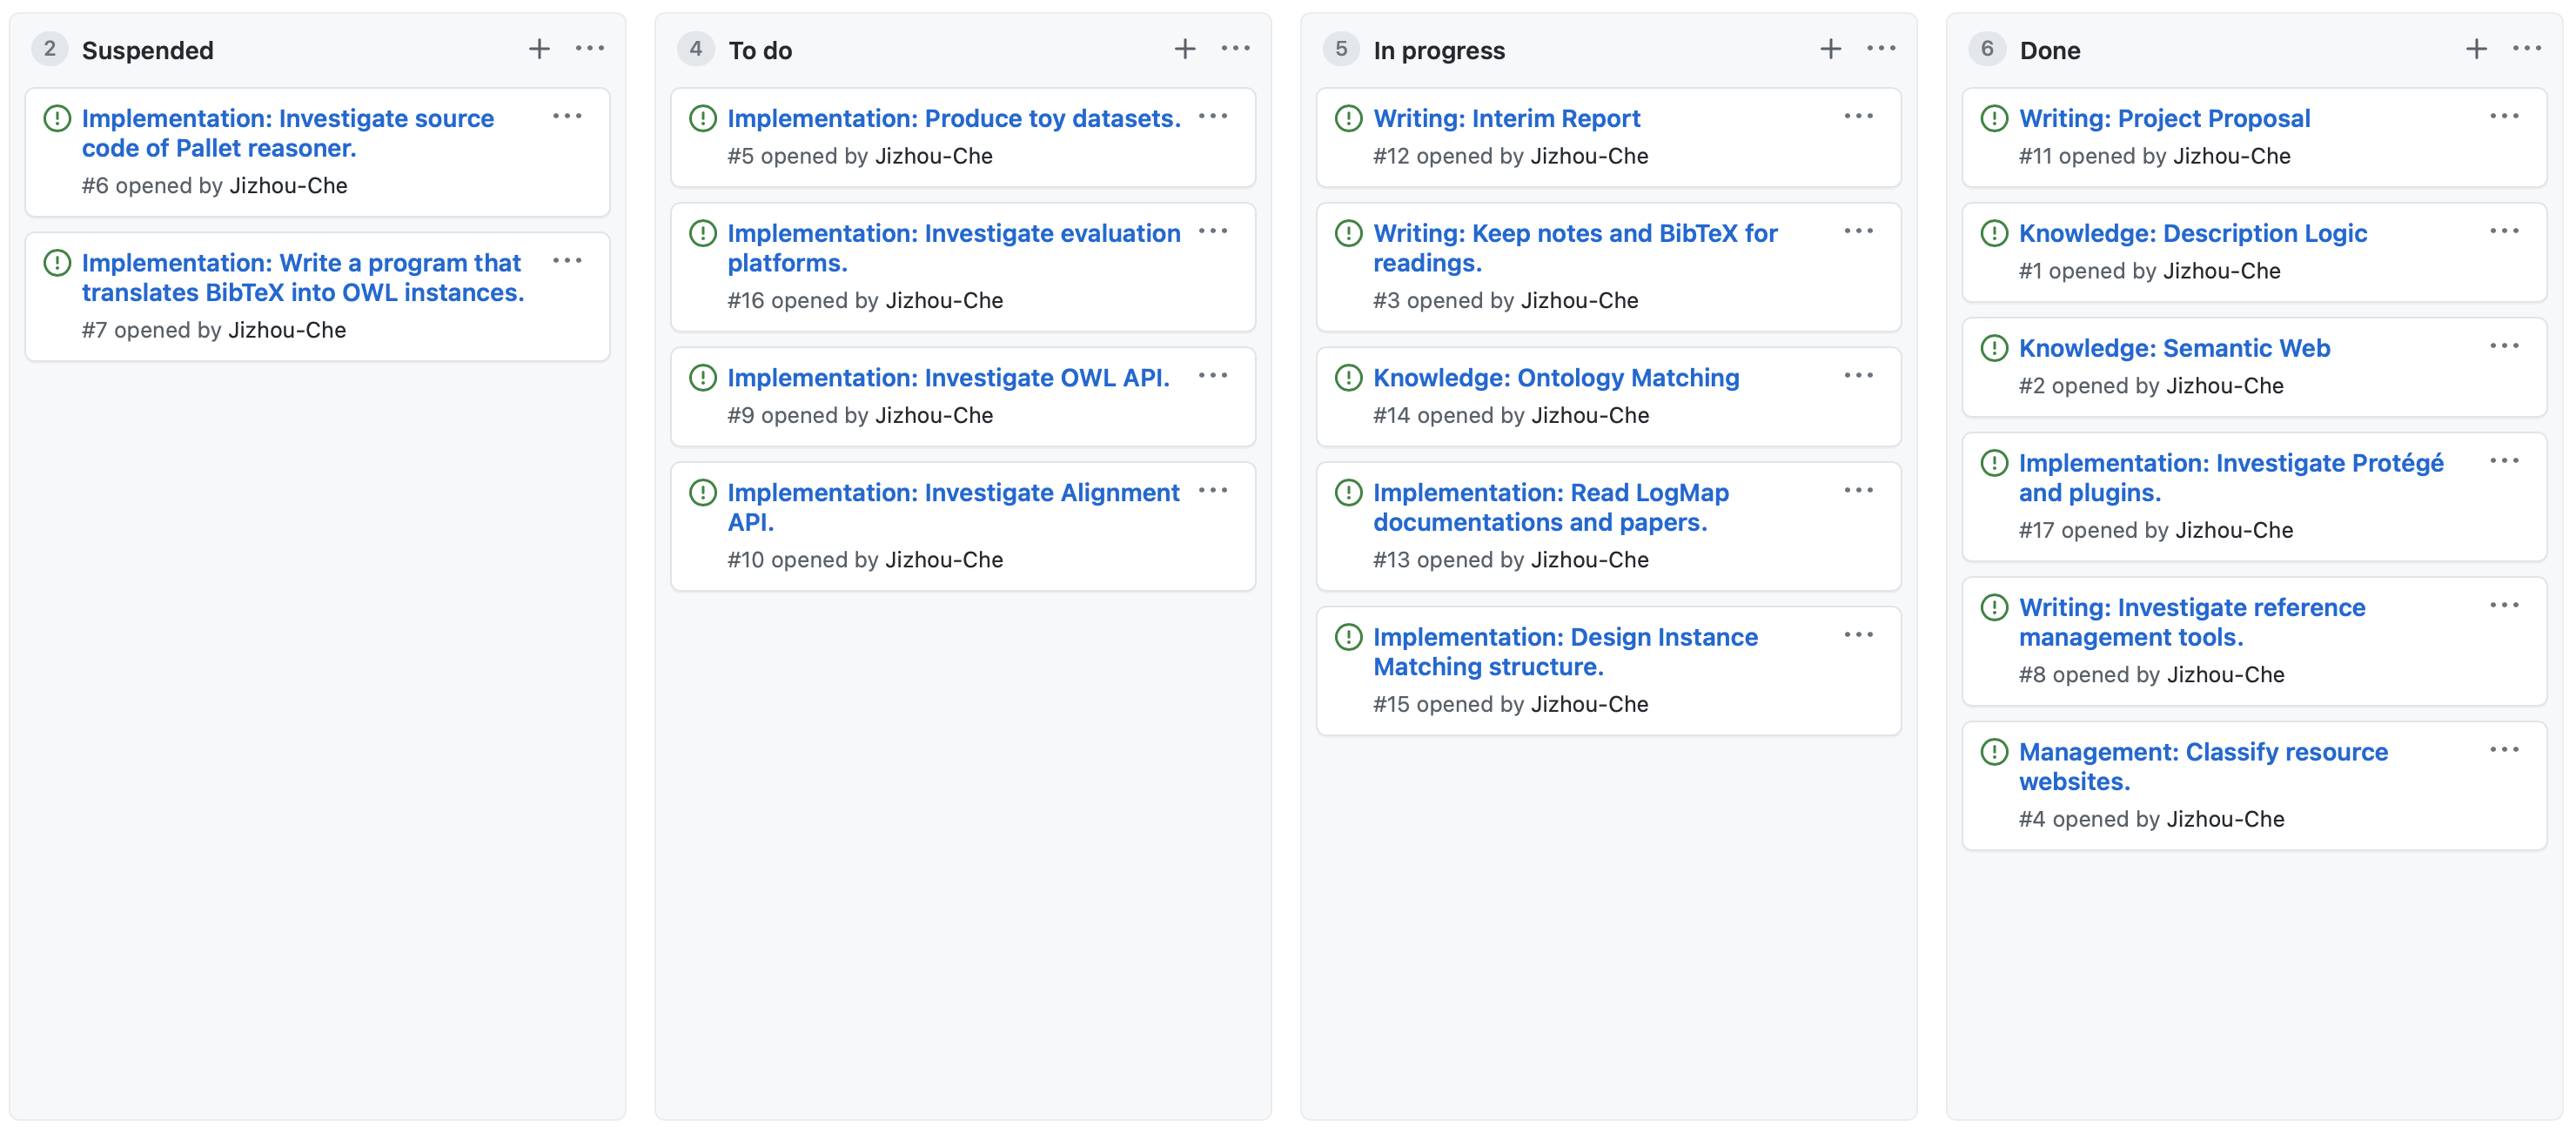
\includegraphics[width=\textwidth]{img/Kanban.png}
\caption{Kanban board}
\label{fig:Kanban}
\end{figure}

\subsection{Resource Management}
% Resource management.
All resources related to the project, such as meeting minutes, reading notes and source code have been managed with the Git version control system and consistently pushed to GitHub. They can be found at \url{https://github.com/Jizhou-Che/Dissertation}. This has proven to be a good practice, in that the evolution of the project is documented within the accumulation and development of resources. The project will stick closely to this methodology during its second half.

\subsection{Contingency Measures}
% Risks that may arise in the revised workplan, and how they can be mitigated and managed.
Admittedly, I didn’t put too much thought into contingency measures at the start of the project. However, I have learned its necessity though my experience in managing this long-term project. Based on the issues I have encountered in the first part of the project as well as my personal observations, the most significant risks that can arise in the process are pointed out below, as well as the proposed strategies to mitigate their effects.
\\\\
Underestimating the steepness of learning curves or the difficulty of implementation can disrupt the regular time allocation, and therefore shake the entire workplan. Apart from foreseeing the issue and allocate adequate amount of time in advance, time can be borrowed from flexible tasks that are less affected by a shrink of timespan. While this provides a temporary solution that mitigates the impact to the workplan, ultimately extra time should be dedicated to the project as compensation.
\\\\
The workloads of other modules is another serious issue, especially when their deadlines are close to the project milestones. This can not only disrupt the time management, but also increase the psychological pressure. Low moods and anxiety can lead to a drop in the productivity as well as the quality of work produced. Having tried the relax-then-focus approach, that was not suitable for me as the guilty only increased. Instead, trying to finish the work together with a friend has proved to be more effective.
\\\\
Offline meetings can sometimes be inappropriate due to wellbeing or other issues. In such cases online meetings via Zoom were organised, and have proven equal effectiveness.


\section{Reflections}
% A personal reflection on the plan and your experience of the project (a critical appraisal of how the project went).

Workplan: original -> changes.
Future directions.
Difficulties and challenges.

I have faced challenges in various aspects of the project. Academically, the steep learning curve of background knowledge made the workload even heavier during the term time that was already intense, and the locating of quality resources required profession judgment and guidance especially at the beginning. My supervisor helped me a lot in such aspects, so I could quickly dive into solid work. Regarding the management of the project, time allocation was the largest difficulty I encountered, as it was hard to balance the project with other curricular subjects, and sometimes my judgment of the amount of time required for a task was inadequate. I consider this as a necessary stage that must be gone through to toughen my skills and enrich my experience, and I feel I have made advancements in my abilities after the first half of the project.
\\\\
During the meetings with my supervisor, I have been taking an orienting role, by preparing relevant materials and questions before the meetings. This made sure that every meeting could go smoothly, and the contents are fully relevant to my working stage at that time. It was an engaging way to gain insights into my performance, and to help me get back on track when I encountered academic or project management difficulties. Thanks to the high quality of the meetings, I can maintain a strong motivation and a high productivity throughout. The meetings were also found to be a good opportunity for both my supervisor and I to know each other better. These are invaluable points and should definitely be kept during the upcoming stages.
